\begin{figure}[H]
    \begin{subfigure}{0.5\linewidth}
        \centering
        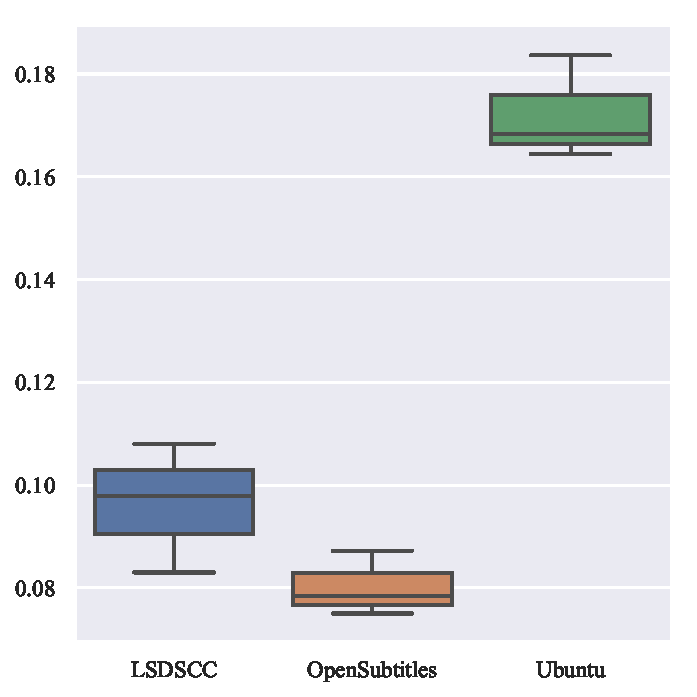
\includegraphics[width=\linewidth]{figure/boxplot/dataset/rouge_1/plot.pdf}
        \caption{ROUGE-1}
    \end{subfigure}%
    \begin{subfigure}{0.5\linewidth}
        \centering
        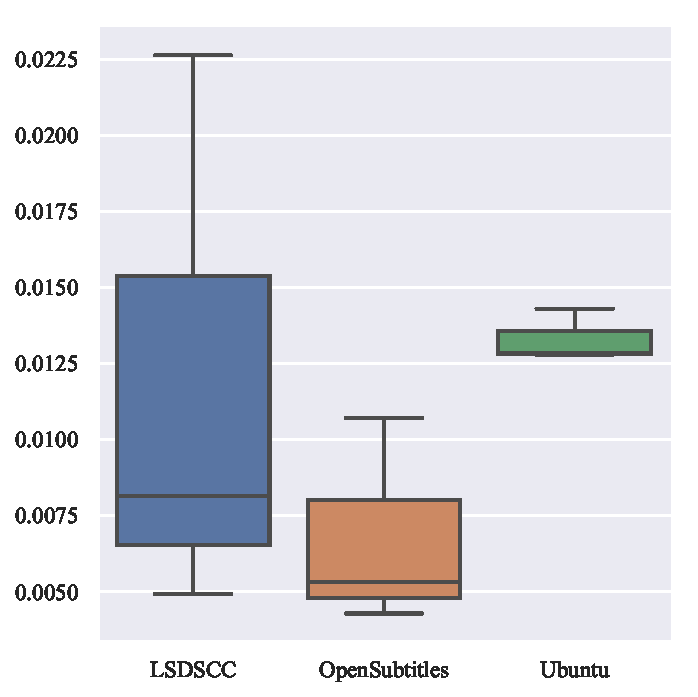
\includegraphics[width=\linewidth]{figure/boxplot/dataset/rouge_2/plot.pdf}
        \caption{ROUGE-2}
    \end{subfigure}
    \begin{subfigure}{0.5\linewidth}
        \centering
        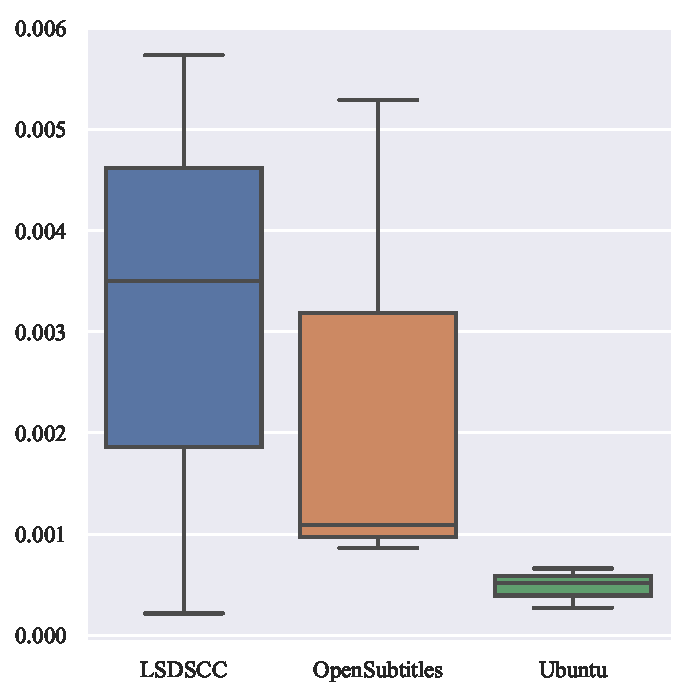
\includegraphics[width=\linewidth]{figure/boxplot/dataset/rouge_3/plot.pdf}
        \caption{ROUGE-3}
    \end{subfigure}%
    \begin{subfigure}{0.5\linewidth}
        \centering
        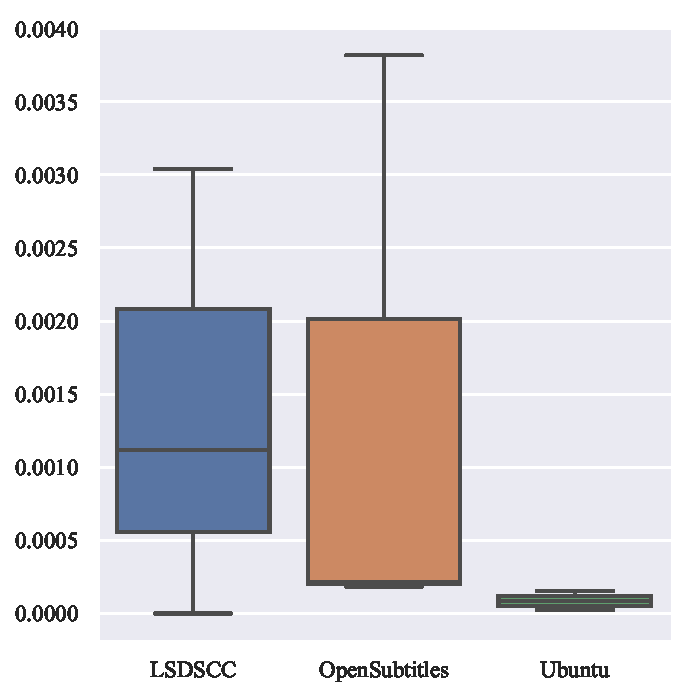
\includegraphics[width=\linewidth]{figure/boxplot/dataset/rouge_4/plot.pdf}
        \caption{ROUGE-4}
    \end{subfigure}
    \centering
    \caption{ROUGE-N的系统得分}
    \label{fig:ROUGE_N_system}
\end{figure}
\begin{figure}[H]
    \begin{subfigure}{0.5\linewidth}
        \centering
        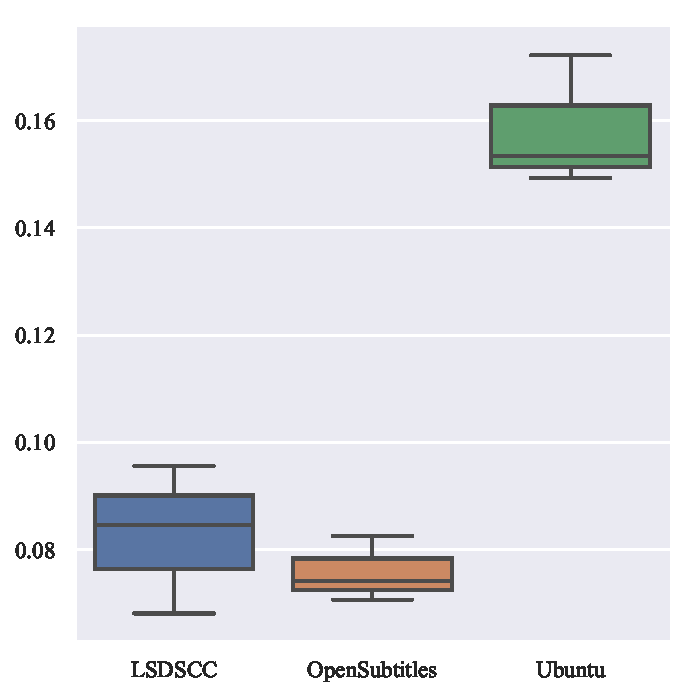
\includegraphics[width=\linewidth]{figure/boxplot/dataset/rouge_l/plot.pdf}
        \caption{ROUGE-L}
    \end{subfigure}%
    \begin{subfigure}{0.5\linewidth}
        \centering
        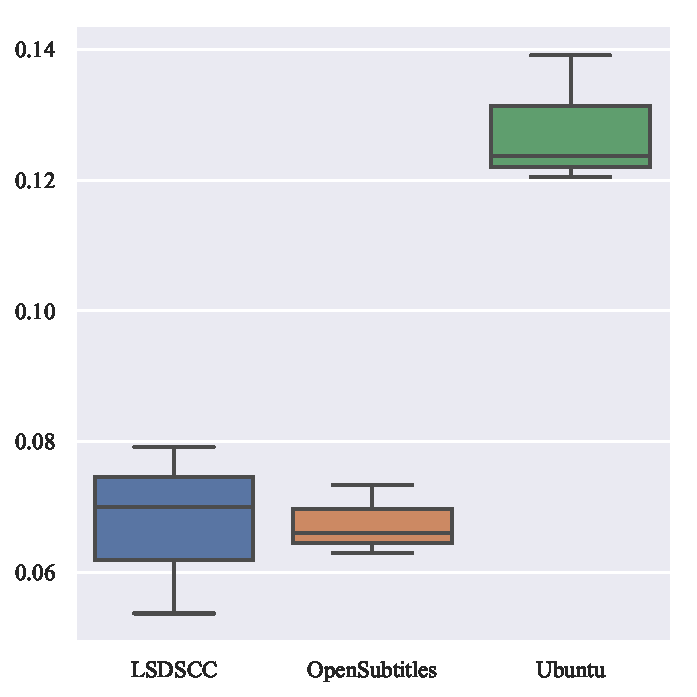
\includegraphics[width=\linewidth]{figure/boxplot/dataset/rouge_w/plot.pdf}
        \caption{ROUGE-W}
    \end{subfigure}
    \centering
    \caption{ROUGE-L和ROUGE-W的系统得分}
    \label{fig:ROUGE_LW_system}
\end{figure}
